\clearpage
\section{SM tW cross section measurement}
\label{App_tW_XS}

In order to do the fit for measuring the tW cross section, we utilize the MLP (which is discussed in Section \ref{signal}) output distributions for both data and MC expectation in the (1jet,1b-jet) and (2jet,1b-jet) regions and event yield in the ($\geq$2jet,2b-jet) region for ee and $\mu\mu$ channels. The inclusion of the ($\geq$2jet,2b-jet) and (2jet,1b-jet) regions helps to constrain the normalization and systematic uncertainties of the \ttbar~ background.

Comparison between observed data and the SM background prediction for the MLP output shape in various jet-bjet regions are shown in Figure \ref{fig:limit_MLP}.
All sources of systematic uncertainties discussed in Section \ref{tW_systematic} are included in our results.

\begin{figure}[ht]
  \begin{center}
    \begin{tabular}{ccc}
      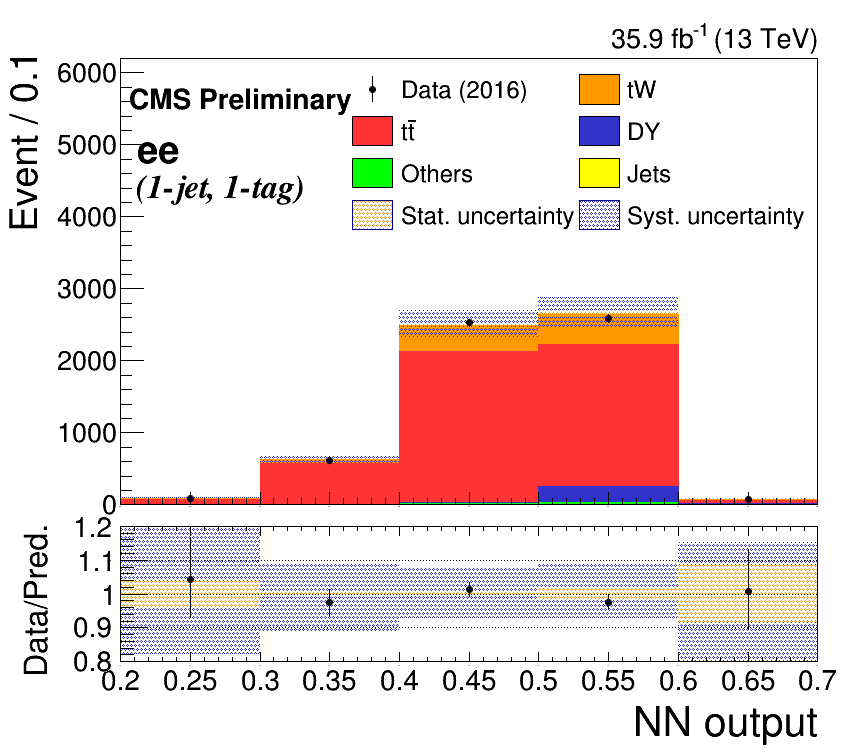
\includegraphics[width=0.4\textwidth]{figures/tW/fig/tW_result/Result/ee/H_MLP_1jet_1bjet.png} &
      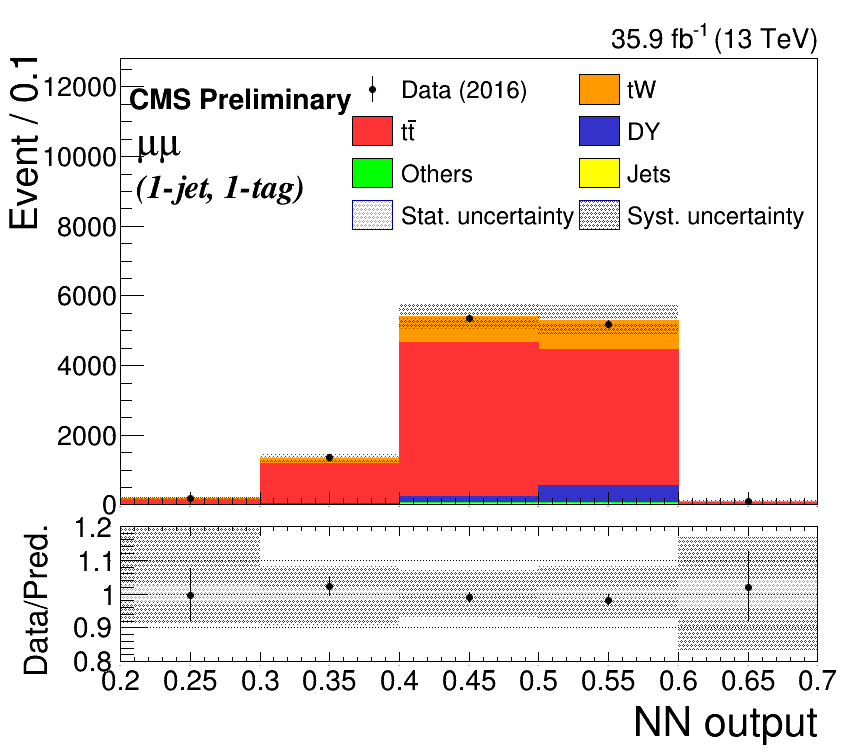
\includegraphics[width=0.4\textwidth]{figures/tW/fig/tW_result/Result/mumu/H_MLP_1jet_1bjet.png}\\
      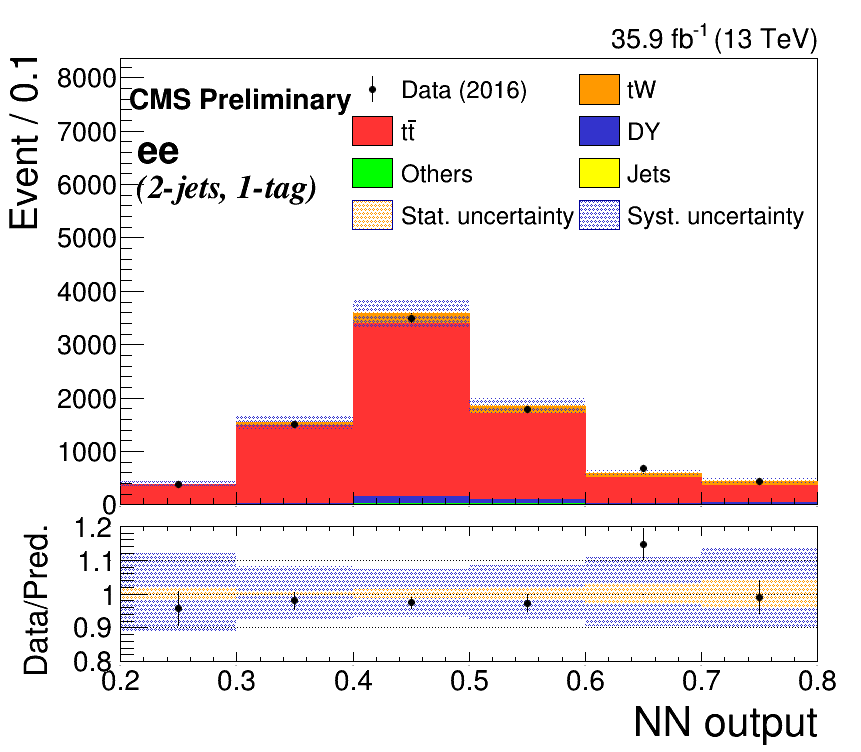
\includegraphics[width=0.4\textwidth]{figures/tW/fig/tW_result/Result/ee/H_MLP_2jet_1bjet.png} &
      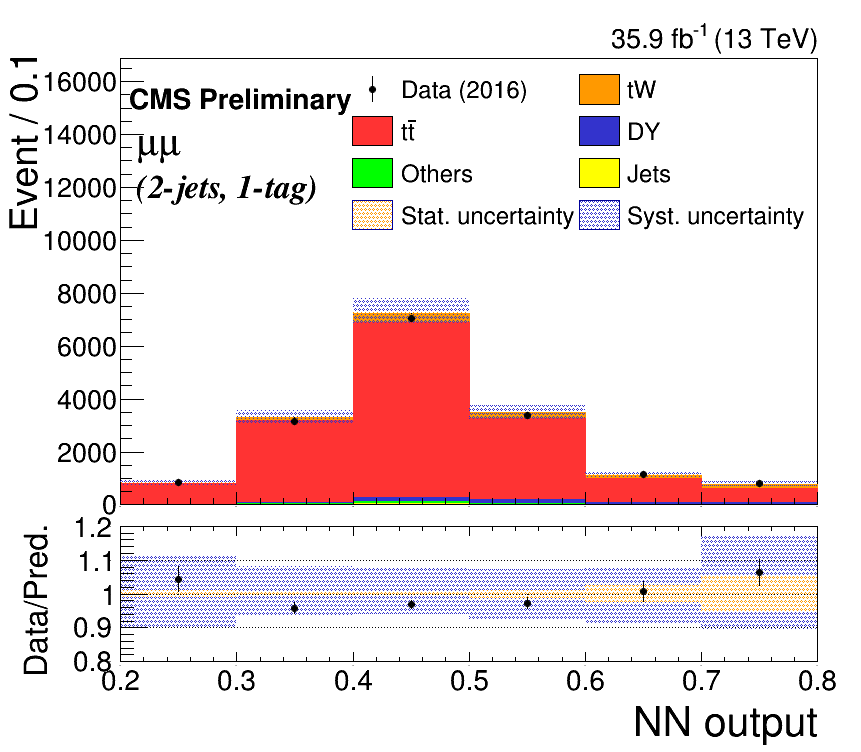
\includegraphics[width=0.4\textwidth]{figures/tW/fig/tW_result/Result/mumu/H_MLP_2jet_1bjet.png}\\
    \end{tabular}
    \caption{The MLP distributions for different (1jet,1b-jet)  region (top row), (2jet,1b-jet) region (bottom row) for $ee$ channel (left column) and $\mu\mu$ channel (right column).
    \label{fig:limit_MLP}}
  \end{center}
\end{figure}

In Figure \ref{fig:scan}, likelihood scan for the signal strength are shown for different region for $ee$ and $\mu\mu$ channels.
In Table \ref{tab:tW_results}, $tW$ measured cross section is reported for $ee$ and $\mu\mu$ channels compared with the result from $e\mu$ channel and combined channels.
In figures \ref{fig:tW_results_part1} and \ref{fig:tW_results_part2}, impact of individual systematic sources for $ee$, $\mu\mu$, $e\mu$ and combined channels are shown for expected and observed.
In Table \ref{tab:uncert_effect}, the effect of each systematic uncertainty source to the combined fit is shown.

\begin{figure}[ht]
  \begin{center}
    \begin{tabular}{cc}
      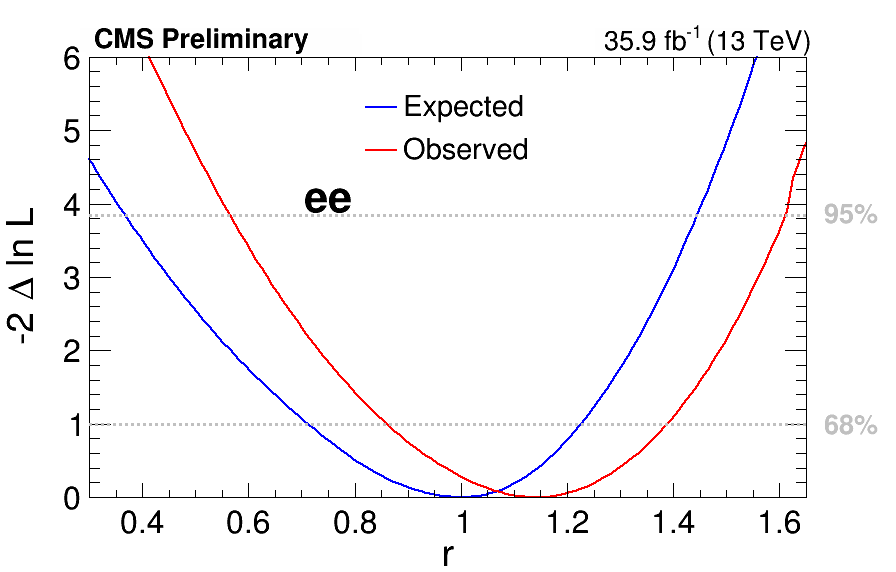
\includegraphics[width=0.45\textwidth]{figures/tW/fig/tW_result/Result/scan_plot/ee__scan.png}
      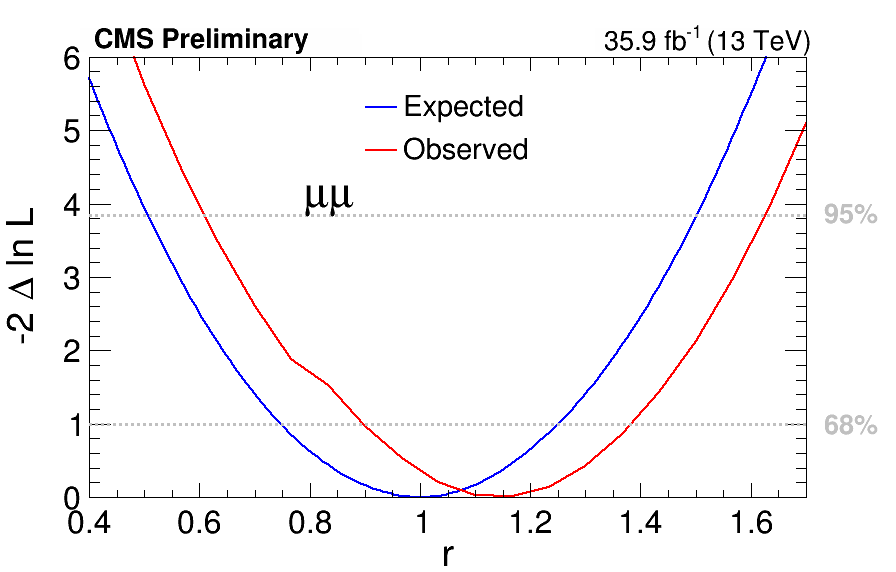
\includegraphics[width=0.45\textwidth]{figures/tW/fig/tW_result/Result/scan_plot/mumu__scan.png}
    \end{tabular}
    \caption{The continue likelihood scan  for various regions for $ee$ channel (left) and $\mu\mu$ (right) channels.
    \label{fig:scan}}
  \end{center}
\end{figure}


\begin{table}[]
\centering
\caption{The expected significance and best fit of $tW$ cross section measurement for $ee$, $e\mu$, $\mu\mu$ channels and combined}
\label{tab:tW_results}
\begin{tabular}{|l|c|c|}
\hline
region                                                          & Exp./Obs. significance $\sigma$      & Exp./Obs. best fit                              \\ \hline
$ee$ MLP output for (1j1t + 2j1t) + yields ($>=$2j,2t)          & 3.2 / 3.5                            & $1.00^{+0.23}_{-0.29}$ / $1.14^{+0.25}_{-0.28}$ \\ \hline
$\mu\mu$ MLP output for (1j1t + 2j1t) + yields ($>=$2j,2t)      & 2.7 / 4.2                            & $1.00^{+0.25}_{-0.25}$ / $1.14^{+0.24}_{-0.27}$ \\ \hline
$e\mu$ MLP output for (1j0t + 1j1t + 2j1t) + yields ($>=$2j,2t) & 6.4 / 5.7                            & $1.00^{+0.14}_{-0.16}$ / $0.92^{+0.16}_{-0.16}$ \\ \hline
combined                                                        & 7.3 / 6.9                            & $1.00^{+0.11}_{-0.12}$ / $0.82^{+0.14}_{-0.12}$ \\ \hline
\end{tabular}
\end{table}




\begin{figure}[ht]
  \begin{center}
    \begin{tabular}{c}
      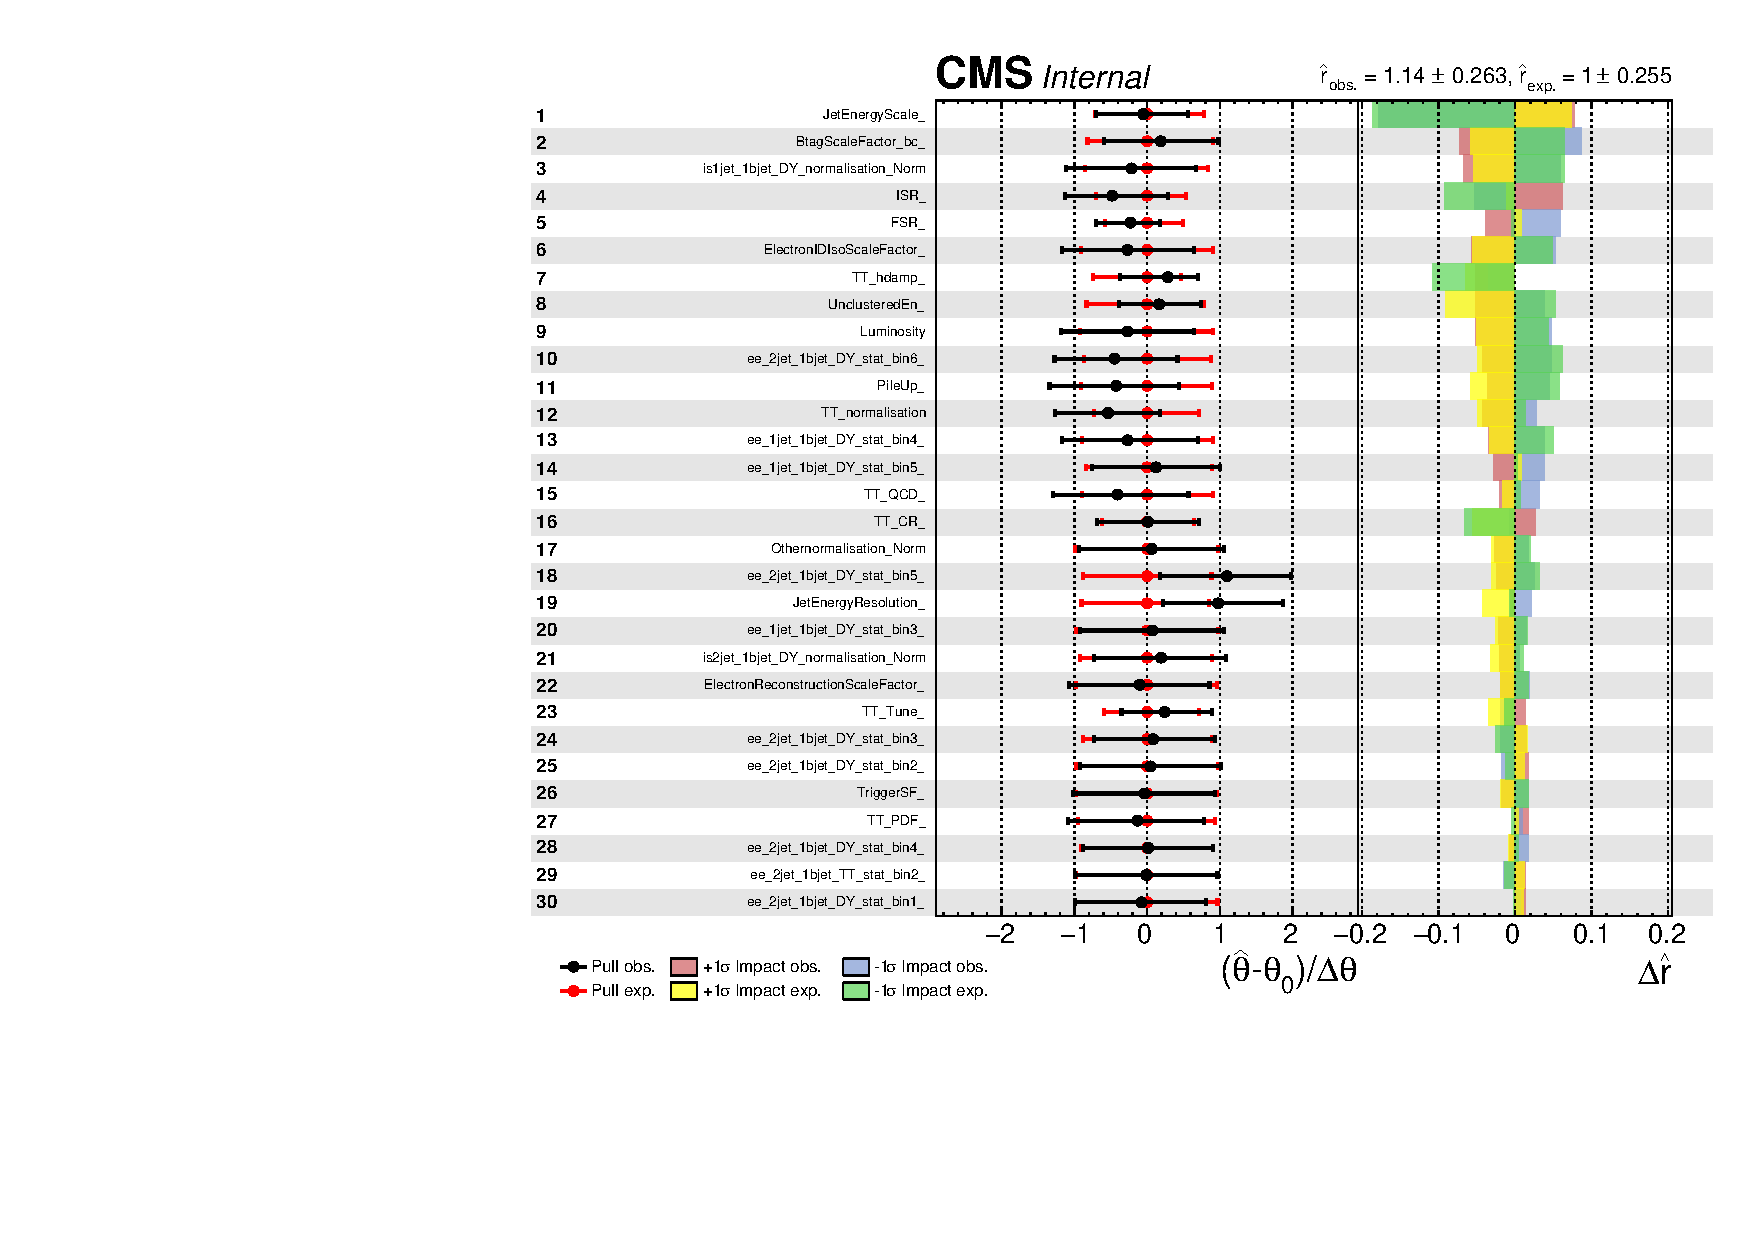
\includegraphics[width=0.9\textwidth]{figures/tW/fig/tW_result/Result/tW_Xsection/ee_card.pdf}\put(-380,320){$ee$}\\
      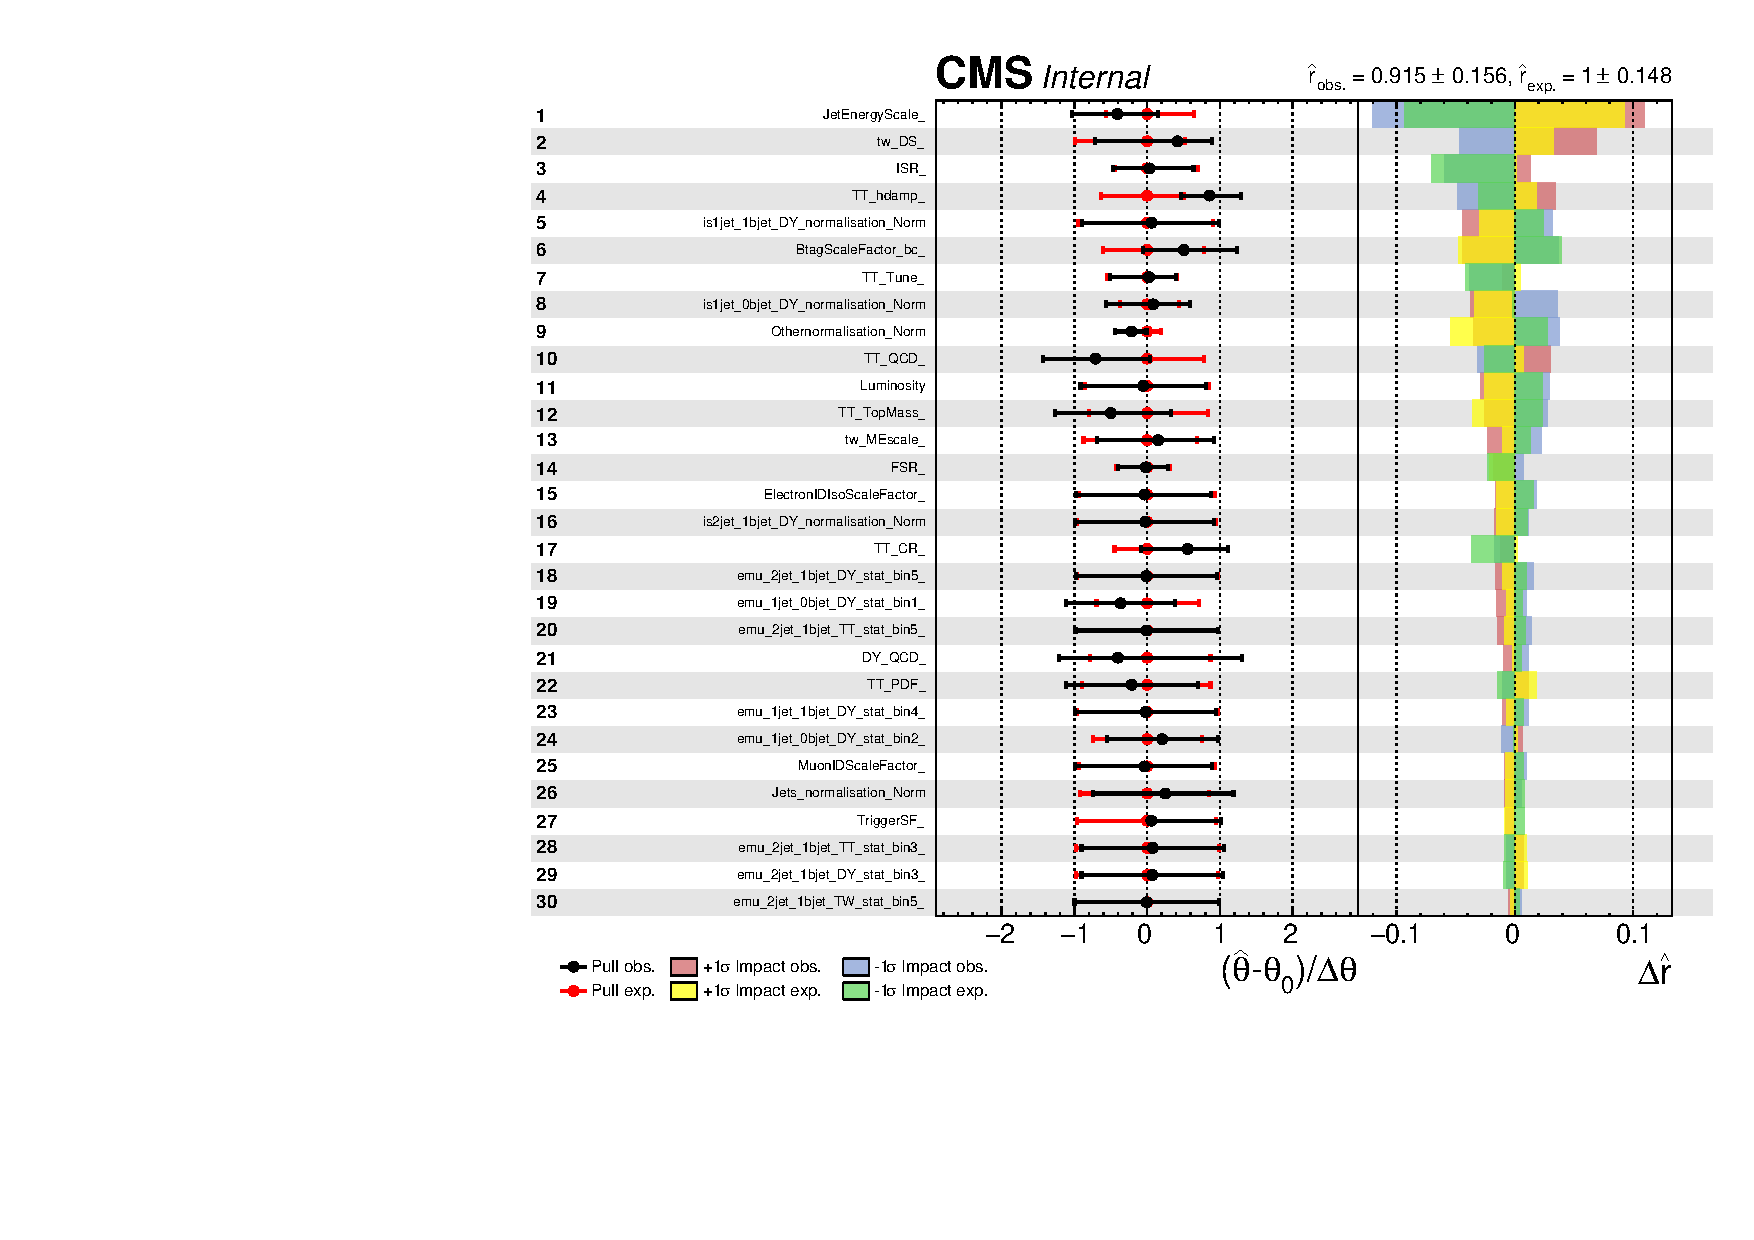
\includegraphics[width=0.9\textwidth]{figures/tW/fig/tW_result/Result/tW_Xsection/emu_card.pdf}\put(-380,320){$e\mu$}\\
    \end{tabular}
    \caption{The expected and observed impacts of the most important uncertainty sources on the measurement of tW cross section in $ee$, $e\mu$ channels.}
    \label{fig:tW_results_part1}
  \end{center}
\end{figure}


\begin{figure}[h]
  \begin{center}
    \begin{tabular}{c}
      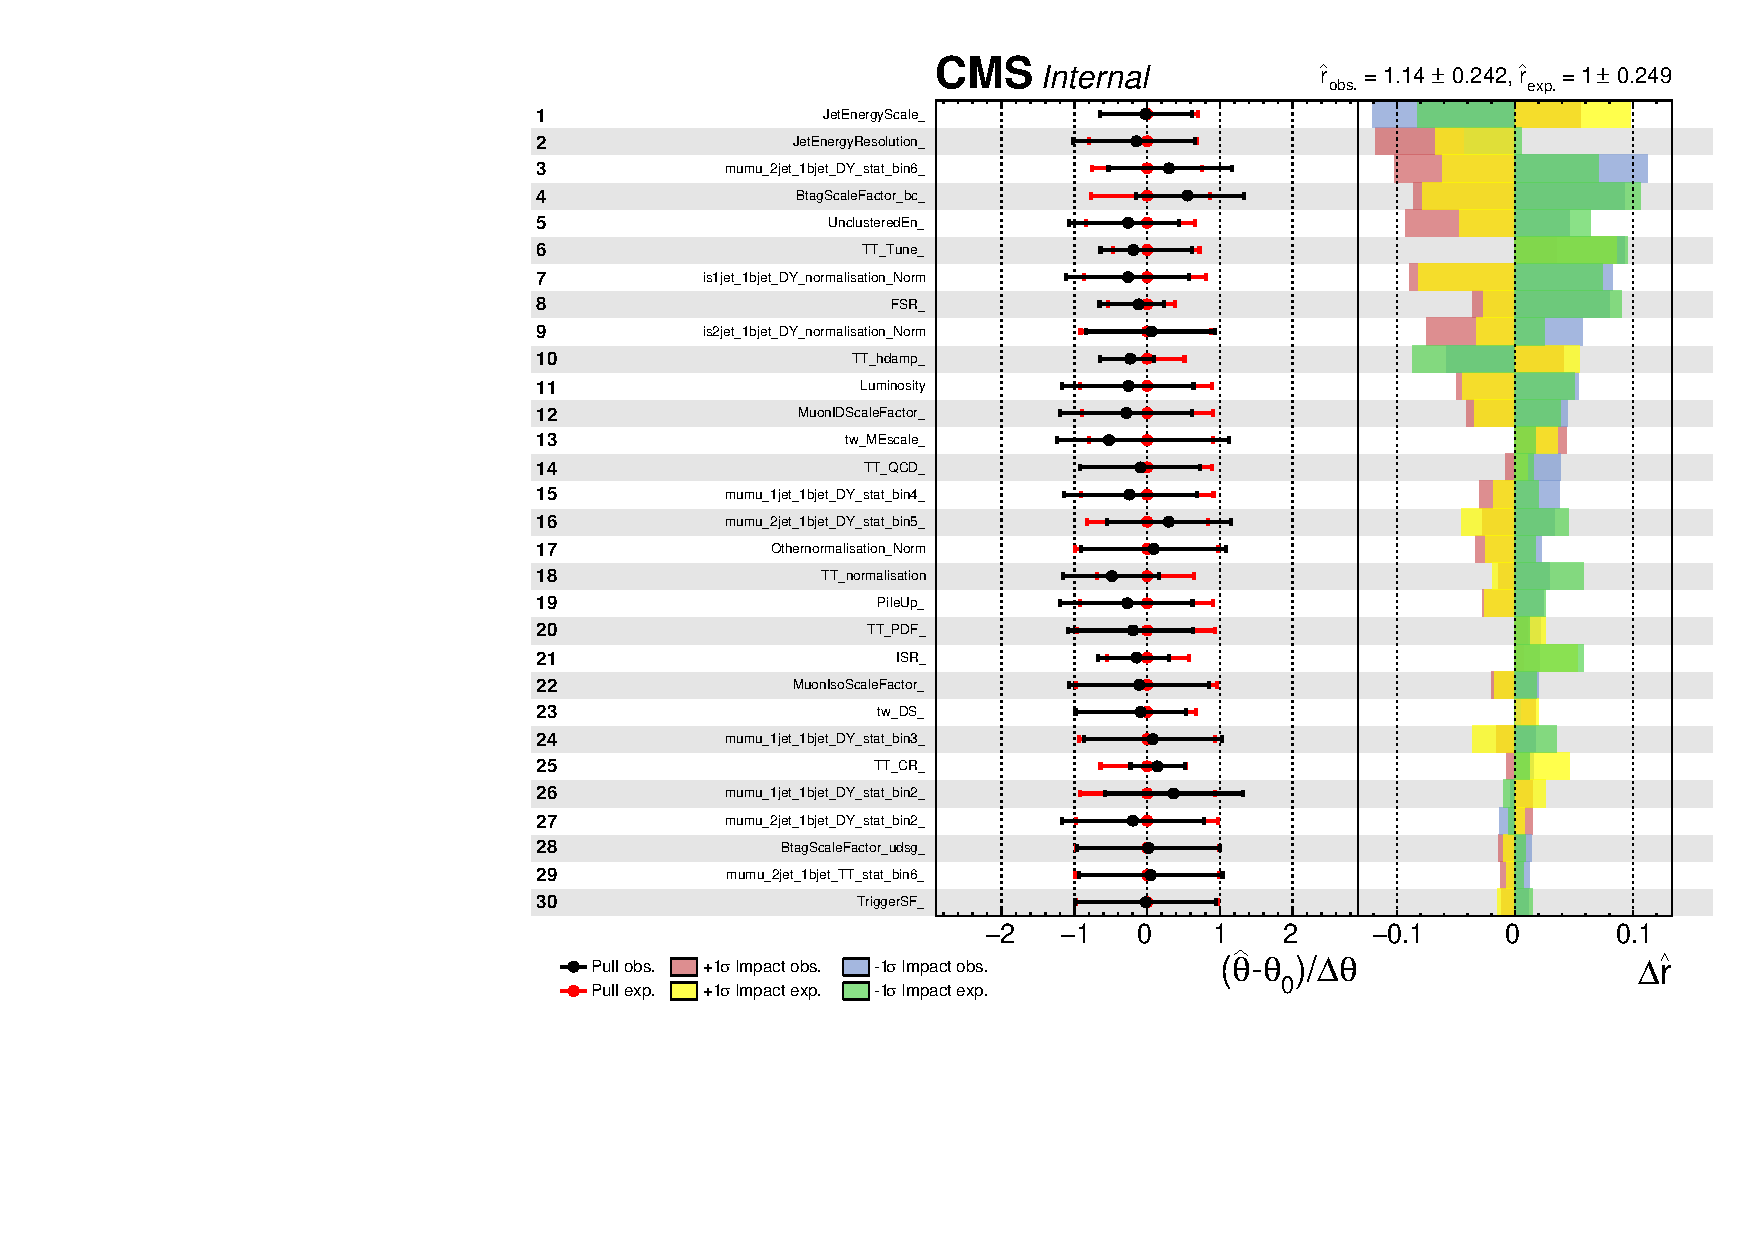
\includegraphics[width=0.9\textwidth]{figures/tW/fig/tW_result/Result/tW_Xsection/mumu_card.pdf}\put(-380,320){$\mu\mu$}\\
      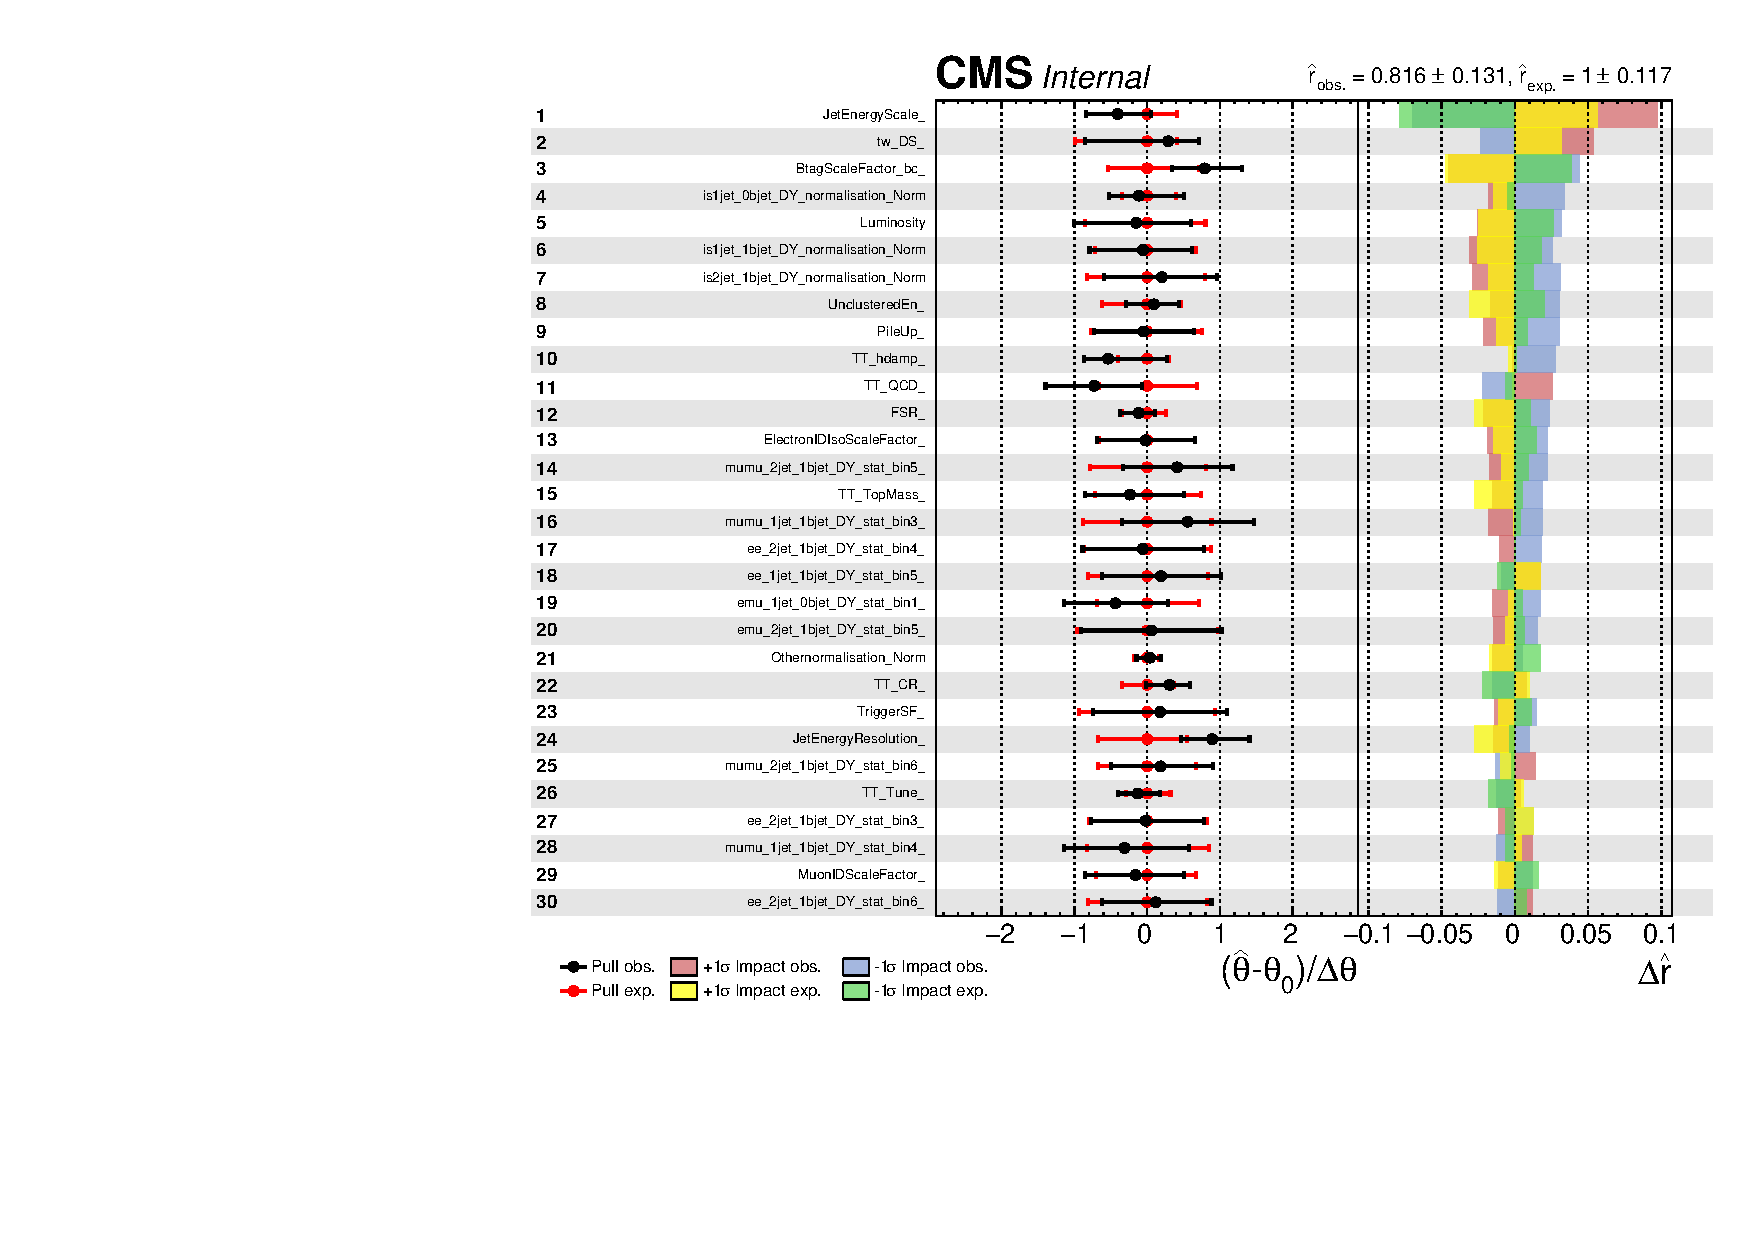
\includegraphics[width=0.9\textwidth]{figures/tW/fig/tW_result/Result/tW_Xsection/ee_emu_mumu_card.pdf}\put(-380,320){Combined}\\
    \end{tabular}
    \caption{The expected and observed impacts of the most important uncertainty sources on the measurement of  tW cross section in  $\mu\mu$ channel and combined.}
    \label{fig:tW_results_part2}
  \end{center}
\end{figure}



\begin{table}[]
\centering
\caption{The effect of systematical uncertainties for combined channel}
\label{tab:uncert_effect}
\begin{tabular}{|c|c|}
\hline
Source & Uncertainty \\ \hline \hline

TT\_PDF & 2.451\% \\ \hline
ISR & 2.734\% \\ \hline
TW\_DS & 8.205\% \\ \hline
FSR & 3.824\% \\ \hline
Trigger & 2.801\% \\ \hline
ElectronIDIso & 3.355\% \\ \hline
PileUp & 3.848\% \\ \hline
TW\_mtop & 1.674\% \\ \hline
DY\_normalisation & 6.578\% \\ \hline
MuonIso & 2.385\% \\ \hline
MuonID & 2.765\% \\ \hline
MuonTrack & 2.015\% \\ \hline
TT\_CR & 3.879\% \\ \hline
Missingtag & 2.608\% \\ \hline
DY\_PDF & 2.569\% \\ \hline
UnclusteredEn & 5.394\% \\ \hline
JER & 3.395\% \\ \hline
JES & 12.475\% \\ \hline
TW\_ME & 2.451\% \\ \hline
Btag & 6.093\% \\ \hline
TT\_QCD & 3.034\% \\ \hline
ElectronReco & 2.698\% \\ \hline
TT\_normalisation & 2.378\% \\ \hline
Other\_normalisation & 3.188\% \\ \hline
TT\_mtop & 2.910\% \\ \hline
TT\_Tune & 3.305\% \\ \hline
DY\_QCD & 1.866\% \\ \hline
Jets\_normalisation & 1.998\% \\ \hline
TT\_hdamp & 3.311\% \\ \hline
Luminosity & 4.431\% \\ \hline
MC\_stat & 6.820\% \\ \hline
Data\_stat & 2.435\% \\ \hline
Total & 16.176\% \\ \hline

\end{tabular}
\end{table}

To summarize, the tW cross-section is measured to be $58.08\pm9.32(syst.)\pm1.43(stat.)~pb$ with a 6.9 (7.3) $\sigma$ significance for observed (expected) and in
agreement with the standard model prediction of $\sigma_{tW}^{ref} = 71.7 \pm 1.8 (scale) \pm 3.4 (PDF)~pb$.

